\chapter[Gestión, planificación y desarrollo del software]{Gestión, planificación y desarrollo del proyecto de software}
Ya hemos introducido las bases del \textit{testing}, de la computación cuántica y de las pruebas de mutación aplicada a la misma. Estamos en disposición de hablar del \textit{software} realizado y que trabaja sobre todos estos conocimientos.

En particular, hablaremos de: gestión, planificación y desarrollo de funcionalidades. La estructura para realizar este capítulo, además de muchos de los conceptos tratados se sustentan en notas de distintas asignaturas de la carrera, especialmente en la asignatura de \textit{Ingeniería del Software}. 
\section{Gestión del proyecto}

En primer lugar vamos a tratar acerca de todo el proceso de gestión del proyecto, desde la organización como equipo, hasta herramientas y \textit{software} utilizado para el desarrollar el código y la memoria.

\subsection{Gestión de equipo}

La gestión del equipo es sencilla, en principio los dos miembros del grupo contamos con el mismo poder para la toma de decisiones y por tanto, dichas decisiones han de tomarse de manera consensuada. Si bien es cierto que, según la actividad, alguno de los miembros puede estar más involucrado en ella y es razonable que sus argumentos tenga un mayor peso.

Además, en caso de decisiones clave siempre teníamos una segunda opinión, correspondiente a nuestro tutor, que por tanto ha formado parte también de la toma de las mismas. Hemos tratado de involucrarnos por igual en todas las fases y tareas del TFG con, tal vez, algunas excepciones. Veremos a continuación de forma detallada la contribución de cada uno al trabajo.

\subsection{Contribución al proyecto de Luis Aguirre}
% Al menos dos páginas

La idea de realizar este proyecto comienza a finales de junio de 2019. Nos pusimos en contacto con el director de este trabajo, Manuel Núñez, y se realiza una primera reunión. Hay que mencionar que las dos disciplinas principales sobre las que se ha construido este trabajo, el mutatation testing y la computación cuántica, son áreas sobre las que no habíamos visto ni si quiera una pequeña introducción en alguna de las asignaturas de la carrera de informática o matemáticas cursadas hasta la fecha.

Es por ello que a raíz de esta reunión inicial surge una primera tarea a realizar: investigar y adquirir conocimiento sobre mutatation testing y computación cuántica. Para ello utilicé como literatura, principalmente, la \textit{Introducción a la computación cuántica para no-físicos}[\cite{rieffel2000introduction}]. De este texto obtuve las primeras nociones importantes sobre computación cuántica que se han ido mencionando a lo largo del texto: qubit, superposición de estados, entrelazamiento, paralelismo y un largo etcétera. Además, también se realizó una lectura exhaustiva de un recurso online [\cite{quantumcountry}] desarrollado por uno de los promotores de la computación cuántica más relevantes en la actualidad, Michael A.Nielsen, y por Andy Matuschak. Este recurso me pareció adecuado pues la interfaz y el método de lectura están construidas sobre potentes ideas del campo de la ciencia cognitiva, y su principal objetivo es hacer que el lector recuerde los nuevos conceptos aprendidos, que en el caso de la computación cuántica suelen tratarse de conceptos y notación que no es familiar.

A su vez, para aprender las primeras ideas del mutation testing se realizó una lectura del artículo \textit{Mutation Testing} [\cite{hierons2010mutation}], si bien más adelante, durante el curso 2019/2020,  decidí cursar la asignatura \textit{Testing de Software} con la idea de ampliar mi conocimiento sobre el testing y de esta forma poder aplicarlo a este proyecto.

Una vez que se tenían las ideas principales sobre computación cuántica y mutation testing se realiza una nueva reunión donde se decide en qué lenguaje cuántico se especializará cada alumno. En mi caso decidí estudiar el lenguaje cuántico de Microsoft: \qsh. Esta tarea implicó aprender a instalar el entorno de desarrollo y las distintas alternativas de las que se disponía, familiarizarse con la sintaxis del lenguajes así como del sistema de tipado, examinar ejemplos de código desarrollado por Microsoft... Esta última tarea fue especialmente importante pues me permitió reconocer que métodos eran más utilizados, siempre con la idea en mente de poder definir un operador de mutación a partir de ellos.

Todo este trabajo es previo a empezar a desarrollar el programa ha sido, posiblemente, la etapa que más tiempo ha consumido. Esto se debe al haber realizado un trabajo sobre un campo que era prácticamente desconocido para ambos, y por ello creíamos que era imprescindible dedicar una importante porción del trabajo a la formación y el estudio de este área.

Tras haber realizado el estudio previo, tarea que se alarga hasta principio de 2020, se comienza con el desarrollo del software. Este proceso se extenderá a lo largo de 3 meses, aproximadamente. La realidad es que ambos componentes del grupo nos hemos involucrado de manera similar en el diseño y creación del programa.

Acostumbrados ya a una dinámica previa de trabajo conjunto, se fueron designando pequeñas tareas que debían ser llevadas a cabo. Este ha sido el proceso que se ha seguido durante todo el desarrollo del software, y por tanto ninguna de las componentes principales del programa ha sido desarrollada única y exclusivamente por alguno de los miembros del grupo.

Sin embargo, la responsabilidad de desarrollar alguna de estas pequeñas tareas mencionadas previamente ha podido recaer en uno de los miembros del grupo, habiendo acordado previamente como debía ser desarrollado, y haciendo una comprobación posterior por parte del otro integrante. Algunas de las tareas, entre otras, que han recaído en mi persona han sido el desarrollo de la lógica encargada del análisis sintáctico del código y la aplicación de los operadores de mutación, el ``parseo'' del código para la obtención de la declaración de todos los métodos involucrados en el programa sobre el que se quiere aplicar pruebas de mutación o una parte relevante de la documentación del código. 

Además, como ya se ha comentado previamente, cada uno de los integrantes del grupo se especializó en un lenguaje de programación concreto, lo que se tradujo en que ciertas clases del programa fueran desarrolladas de manera exclusiva por cada miembro del grupo. Estas clases son las relacionadas de manera directa con cada lenguaje de programación. 

En particular, encontramos las clases usadas parar definir cada operador de mutación. Además, en el caso de \qsh, tuve definir ciertas expresiones regulares que me permitían analizar el código en busca de cadenas de caracteres de una manera más precisa. También recayó sobre mi la especificación de la entrada por parte del usuario para el lenguaje \qsh, así como la generación automática del script de Python encargado de llamar a las subrutinas de \qsh a las que se deseaba aplicar las pruebas de mutación.

Por último, en lo relativo a la elaboración de esta memoria, si que se ha realizado un reparto de tareas más amplio. Esto se debe a que, tras realizar un reunión previa donde se decidió la estructura de la memoria, se dio con una distribución de capítulos los cuales eran prácticamente independientes unos de otros. La división del trabajo individual por capítulos nos iba a permitir trabajar de manera más rápida. 

El capítulo dedicado a la introducción del testing y las pruebas de mutación se decidió que fuese mayormente desarrollado por mí, ya que contaba con un poco más de experiencia en dicho ámbito tras haber cursado la ya mencionada asignatura \textit{Testing de Software} a lo largo de este mismo año. Además, al manejar con mayor soltura el idioma anglosajón que mi compañero, he sido el encargado de traducir los capítulos que debían ser añadidos a esta memoria también en inglés.

Así, si bien ciertas tareas se han realizado de manera individual a lo largo de este proyecto, siempre ha habido previamente una puesta en común de ideas, así como una comprobación posterior por parte de ambos integrantes para de esta forma asegurar que, tanto Javier como yo, quedáramos satisfechos, bajo nuestros estándares individuales, del trabajo realizado.

\subsection{Contribución al proyecto de Javier Pellejero}
% Al menos dos páginas

En primer lugar, y como detallaremos en las secciones venideras, cabe destacar la dedicación empleada a adquirir los conocimientos necesarios para poder realizar este TFG. A la hora de hablar de temas como planificación o el estudio de los temas tratados, es difícil separar el trabajo realizado para los TFG de las facultades de matemáticas e informática.

Así, nuestra base sobre pruebas de mutación y computación cuántica eran mínimas, pero además, hay que destacar que en este texto se omiten muchas cuestiones más profundas, relevantes al mundo de la mecánica cuántica y sus pilares matemáticos y que sí he creído convenientes relatar en el TFG del grado de matemáticas. De este modo, quiero destacar que la preparación para poder realizar ambos trabajos ha sido laboriosa, ha ocupado una parte muy significativa del tiempo total empleado y que no siempre se manifiesta fácilmente este esfuerzo en las memorias realizadas.

La primera toma de contacto con el mundo de la computación cuántica fue mediante \textit{An Introduction to Quantum Computing for Non-Physicists} [\cite{rieffel2000introduction}] recomendado por nuestro tutor. Desde mi punto de vista es un contenido muy completo, con multitud de referencias y ejemplos y útil para adentrarse en los sistemas de información cuánticos. Sin embargo, su título refleja la ausencia de contenido referente a las bases en las que se sustenta todo este marco teórico y si se quiere profundizar sobre ellas se debe acudir a otras fuentes más completos.

La solución a este problema tiene por nombre \textit{Quantum Computation and Quantum Information} [\cite{nielsen2001quantum}]. Ha sido mi principal referencia a la hora de ahondar en la experiencia cuántica. Dedica muchas páginas a construir desde cero todo el marco matemático que sustenta la este tipo de computación desde nociones tan básicas como espacios vectoriales, a otras algo más elaboradas como ciertas propiedades de los espacios de \textit{Hilbert}. Aún así, aunque también dedica numerosas páginas a entender los entresijos de los postulados cuánticos, no es todo lo completo que debiera ser.

En cuanto al \textit{mutation testing}, el artículo de nuestro tutor con otros colaboradores [\cite{hierons2010mutation}] fue nuestra iniciación en esta modalidad de test con respecto a la computación clásica. La adaptación cuántica fue un proceso que se desarrolló principalmente bajo las indicaciones de nuestro tutor y las contribuciones de otro referentes [\cite{usaolaquantum}] con la intervención de nuestras propias ideas.

Mientras adquiría estos conocimientos me iba familiarizando con el lenguaje en el que profundizo en el TFG de matemáticas, \textit{Qiskit} de IBM. Aunque su documentación es extensa, existen herramientas importantes que carecen de ella. En cuanto a la sintaxis, es fácil de aprender y legible. Además, pese a que el hecho de pensar en puertas cuánticas podría convertirlo en un lenguaje de nivel inferior a uno ensamblador clásico, el estar combinado con un lenguaje de alto nivel multiparadigma como \textit{Python} hacen un mundo de posibilidades, muchas de ellas aún por explotar.

El número de ejemplos de código en \textit{Qiskit} presente en Internet no es abundante, pero permite hacerse a la idea de qué instrucciones son las más usadas y por tanto las más propensas a sufrir equivocaciones por parte del programador.

En cuanto al proyecto de \textit{software}, la involucración de ambos miembros del grupo trató de ser lo más pareja posible. Sin embargo, debido a mi conocimiento sobre \textit{Qiskit}, me encargué de elaborar todos sus operadores de mutación, la estructura de entrada de datos a modo de ejemplo que será comentada más adelante en este capítulo y todo el proceso referente a las llamadas a \textit{Python} que ejecutan las pruebas de mutación sobre \textit{Qiskit}.

Además, tuve cierto peso adicional a la hora de establecer la estructura del código \textit{Java}  constituida por todas las clases, paquetes o patrones de diseño que acaban marcando las funcionalidades del programa. También estuve centrado en la estructura de la mayoría de las vistas y las herramientas visuales creadas para ellas o el desarrollo de ciertos paquetes de la lógica, pero siempre con la supervisión de mi compañero Luis.

Podemos asegurar que no hay parte del código en la que no hayamos estado involucrados y por tanto, que desconozcamos su funcionamiento por mucho que dichas líneas estuvieran escritas por el otro miembro del grupo.

En cuanto a esta memoria, si se ha planificado de forma más especializada. A nivel de documento no solamente es complicado, sino que carece de sentido estar trabajando sobre las mismas líneas del archivo. Pese a ello, el capítulo 2 referente a la introducción a la computación cuántica y el último, de ejemplos y conclusiones, han sido elaborados de manera conjunta, dividiendo el trabajo por secciones y subsecciones.

En mi caso, pero siempre de manera planificada y supervisada por mi compañero, me he encargado del capítulo en el que nos encontramos debido a mi ligero mayor peso y toma de decisiones en la estructura del \textit{software}. Como veremos a continuación, explico nuestra planificación, modelo de proceso, pero sobre todo, todo lo referente a las funcionalidades del programa, la estructura del código, que partes del mismo influyen en cada uso del programa, etcétera.

En conclusión, quiero destacar el esfuerzo de ambos componentes del equipo para desarrollar este proyecto del cual espero que tenga continuidad. Creo que las herramientas que hemos proporcionado pueden ser útiles para algunos investigadores que están tratando de dar cada vez más importancia al \textit{testing} en la computación cuántica y pueden ser mejoradas y desarrolladas por otros colaboradores y estudiantes en futuros proyectos.

\subsection{Gestión de configuración}

Hablemos ahora de todas las herramientas y elementos de \textit{software} utilizados para el proyecto. Empezando por esta memoria, al estar realizada en \LaTeX, hemos necesitado programas para su edición y compilación. Ambos componentes del grupo hemos utilizado como distribución \textit{MiKTeX}, mientras que como editor hemos usado \textit{Texmaker}.

En cuanto al \textit{software}, el grueso del programa está realizado en \textit{Java} y es utilizado como gestor y editor del mismo la plataforma \textit{Eclipse} usando como herramienta de desarrollo la octava versión \textit{Java SE Development Kit} (JDK) de \textit{Oracle}.

El programa principal debe realizar una serie de test sobre los lenguajes de computación cuántica \qsh\ y \textit{Qiskit}. En el caso del primero, permite ser llamado desde \csh\ y {Python}, siendo más común utilizar el primero. En el caso del segundo, más que un lenguaje en sí mismo, es un marco de trabajo que engloba varias librerías que se ejecutan sobre \textit{Python}. Se opta por dejar \csh\ de lado, puesto que \textit{Python} es el lenguaje en común de ambos, y que nuestro programa principal, mediante una llamada a sistema, ejecute un programa en dicho lenguaje.

Este programa cambia con cada ejecución y es el programa en \textit{Java} principal quien debe escribirlo. Sin embargo, se han de escribir archivos adicionales en \textit{Python} que contienen funciones útiles y siempre necesarias y para ello se emplea un programa de edición sencillo como \textit{Notepad++}, además de \textit{Jupyter Notebook}, usando la distribución \textit{Anaconda}, para verificar que nuestras funciones escritas tanto por nosotros como por el programa funcionan correctamente.

Para el correcto funcionamiento del programa en su conjunto, se necesitan una serie de requisitos.

\begin{itemize}
\item Una máquina virtual capaz de ejecutar \textit{Java} como \textit{Java Runtime Environment} (JRE).
\item \textit{Python} 2 o 3. (Se recomienda \textit{Python} 3).
\item La librería de \textit{Python} \textit{func-timeout} de Tim Savannah bajo licencia LGPLv3 accesible en \textbf{https://github.com/kata198/func\_timeout/blob/master/LICENSE}. Se adjunta en el repositorio del proyecto.
\item \qsh\ (sólo si se realizaran test con este lenguaje cuántico).
\item \textit{Qiskit} (sólo si se realizaran test con este lenguaje cuántico).
\end{itemize}

En cuanto a la organización y distribución de nuestro código, hemos elegido \textit{Github}. Además de ser un excelente gestor de versiones, tiene el programa (para el sistema operativo\textit{Windows}) \textit{Github Desktop}, una interfaz sencilla para subir y gestionar el código. En el repositorio existen dos carpetas principales en el directorio raíz:

\begin{itemize}
\item \textbf{tex}: que almacena el código \LaTeX.
\item \textbf{src}: que almacena el código, tanto \textit{Java} como \textit{Python}
\end{itemize}

Además existen otras carpetas de menor relevancia con contenidos como ejemplos en los dos lenguajes cuánticos tratados, presentaciones, además de encontrarse en la raíz principal la \textbf{licencia MIT}.

Como veremos, este programa no sólo puede ser realmente utilizado por cualquier interesado en realizar pruebas de mutación sobre programas cuánticos, sino que pueden ser integradas una serie de funcionalidades adicionales en el mismo. Por ello hemos optado por esta licencia, que posiblemente sea la de menor número de restricciones. Cualquiera puede tomar el proyecto y modificarlo, incluso para uso comercial.

\section{Planificación}

La planificación del proyecto puede dividirse en dos aspectos: uno desde el punto de vista temporal que incluye el proceso de investigación, \textit{software} y la realización de la memoria; y otro desde el punto de vista del modelo de proceso elegido para el \textit{software}.

\subsection{Planificación temporal}

Para planificar este Trabajo de Fin de Grado es importante entender que, como alumnos del doble grado en ingeniería informática y matemáticas, debemos realizar un TFG por grado. Nuestra idea inicial es que ambos trabajos estuvieran relacionados y ya en julio contactamos con nuestro tutor y conocíamos el tema de los mismos.

Dejamos constancia de que en el caso del TFG de matemáticas, dichos trabajos eran individuales aunque ambos alumnos tratamos un tema común que es el de introducirnos en la computación cuántica con una sólida base matemática y con alguna pincelada de conocimiento en mecánica cuántica. Además, cada uno introduce un lenguaje de programación cuántico: \qsh\ en el caso de Luis Aguirre y \textit{Qiskit} en el caso de Javier Pellejero.

Por tanto, se puede argumentar que este trabajo tiene sus cimientos en los dos realizados por cada miembro del grupo para el grado de matemáticas. Explicado esto, empezaremos por enumerar una serie de fases de planificación que incluye todos los trabajos.

\begin{enumerate}
\item \textbf{Proceso de investigación}. Puesto que se trata de una serie de conocimientos totalmente nuevos para nosotros y con una complejidad considerable, es importante dotar a esta fase de una duración prolongada. Decidimos establecer como límite para esta fase finales de enero coincidiendo con el fin de exámenes del primer cuatrimestre. En el segundo, ninguno de los integrantes del grupo tiene otras asignaturas, así que hay tiempo suficiente para el resto de fases.
\item \textbf{Desarrollo del \textit{software}}. Una vez familiarizados con la teoría de la computación cuántica y de pruebas de mutación, estamos en condiciones de comenzar nuestro programa. En las siguientes páginas se dará más detalle del mismo. En cuanto al tiempo, estimamos unos dos meses, febrero y marzo, para realizarlo.
\item \textbf{Memorias individuales del TFG del grado de matemáticas}. Por lo comentado anteriormente, es consecuente realizar primero estas memorias pues su contenido sirve de base para desarrollar esta misma. Se estable que el tiempo marcado por el mes de abril es apropiado para realizarla.
\item \textbf{Memoria del TFG del grado en ingeniería informática}. Siguiente tarea a efectuar. Prevista para el mes de mayo.
\item \textbf{Revisión}. Se establece el mes de junio para ultimar memorias, perfección del \textit{software} o cualquier otra tarea que pudiera no estar acabada.
\end{enumerate}

Aclaramos que estas fechas son orientativas. Como veremos a continuación, nuestro modelo de proceso del \textit{software} se asemeja a un \textbf{desarrollo evolutivo ágil}, concretamente al denominado \textbf{\textit{eXtreme Programming}} (XP) y sus principios pueden aplicarse también a toda la planificación anterior. Puesto que el tiempo no parece un problema determinante, no seremos estrictos con las fases anteriormente mencionadas.

\subsection{Modelo de proceso}

Acabamos de comentar el modelo en el que se basa nuestro desarrollo del programa. Creemos poder dar algunos buenos argumentos de por qué es una buena decisión. Al contar con un grupo de tan solo dos integrantes, la comunicación entre ambos es clara, concisa y rápida, no sólo entre nosotros sino también con el tutor (al que podemos asignar el rol de cliente), lo que ayuda a prevenir malentendidos que acaban en errores y problemas difíciles de vaticinar aún con un proceso de desarrollo pesado con una planificación más exhaustiva como el proceso unificado.

Otro factor a tener en cuenta es que, si bien los conceptos sobre los que trata nuestro programa no son elementales, no es excesivamente complejo el hecho de implementarlos. Además, al ser un área de la computación en el que no se ha investigado aún en exceso, puede surgir en cualquier momento la necesidad de cambios o implementar nuevas funcionalidades.

El uso de XP facilita este último hecho, pues intercala continuamente diseño y desarrollo de manera evolutiva e iterativa. En nuestro caso, es muy importante disponer de una versión ejecutable del programa desde el momento que esté desarrollada la primera funcionalidad, lo cual hemos logrado. Para ello, diseñamos una vista, le damos forma mediante código y la ensamblamos con la lógica. Antes de continuar una nueva vista, nos aseguramos que la funcionalidad implementada tiene una correcta actividad para evitar el encadenamiento de errores.

%------- Figura iteración XP
\begin{figure}[!htb]
\begin{center}
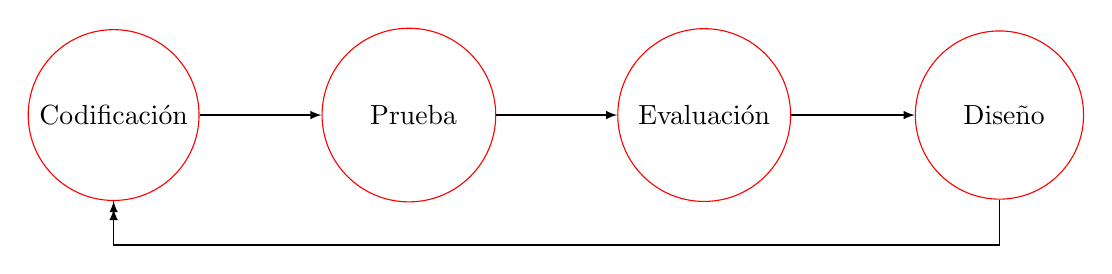
\begin{tikzpicture}[x=1.5cm, y=1.5cm]
	%\fill (-3.2,0) circle (0.1pt)node[anchor=east] {$20$};
	%\fill (3.2,0) circle (0.1pt)node[anchor=west] {$-20$};
    \node[circle,draw=red] (v1) at (-3.75,0) {Codificación};
    \node[circle,draw=red] (v2) at (-1.25,0) {\ \ \ \ Prueba\ \ \ \ };
    \node[circle,draw=red] (v3) at (1.25,0) {\ Evaluación\ \ };
    \node[circle,draw=red] (v4) at (3.75,0) {\ \ \ \ Diseño\ \ \ \ };
    \draw[color=black, -latex]  (v1) edge (v2);
    \draw[color=black, -latex]  (v2) edge (v3);
    \draw[color=black, -latex]  (v3) edge (v4);
    \draw (v4) -- (3.75,-1.1) -- (-3.75,-1.1) -> (v1);
    \draw[color=black, -latex]  (-3.75,-0.795) edge (v1);
\end{tikzpicture}
\end{center}
\caption{Iteración de etapas en XP.}
\label{fig:fig1}
\end{figure}

En la figura \ref{fig:fig1} podemos observar un diagrama de las etapas estándar de XP. Si bien la primera etapa se corresponde normalmente con la codificación, en nuestro caso siempre lo ha sido el diseño. Así, para cada funcionalidad, se diseña la vista, se implementa la misma, a continuación se desarrolla y enlaza la lógica y por último se prueba. Se itera sobre estas etapas para cada vista y funcionalidad establecidas.

Se sigue así una planificación diseñada prácticamente para cada funcionalidad (planificación incremental) marcándose objetivos a muy corto plazo pero sin perder de vista el objetivo final: completar el programa y su correcto funcionamiento.

Para concluir, hemos tratado de hacer nuestro código lo más adaptable posible, no sólo por el tipo de proceso de desarrollo elegido, sino también para facilitar futuras implementaciones de nuevas funciones para el programa. Esto, sumado a todo lo contado en los anteriores párrafos, justifica que nuestro proceso de desarrollo se ajuste a XP y su correcta elección.

\section{\textit{Mutation Testing for Quantum Computing} (MTQC)}

MTQC son las siglas que dan nombre a nuestro programa. Su principal funcionalidad es la de aplicar pruebas de mutación en distintos lenguajes cuánticos, en nuestro caso \qsh\ y \textit{Qiskit}.

La secuencia de acciones de un usuario en poder de MTQC sería la de generar mutantes del programa deseado, verificar el resultado de los mutantes creados, ejecutar el programa original y los mutantes seleccionados dadas una serie de test y cotejar los resultados para encontrar test satisfactorios e indeseados.

Sobre estas cuatro fases hemos establecido toda nuestra planificación, análisis y diseño del proyecto y es así como vamos a explicar todo el proyecto, tomando estas etapas como estructura de cara al desarrollo.

\subsection{Principales funcionalidades}

Aunque el desarrollo dirigido por casos de uso no es propio de XP, nos inspiramos en ellos para determinar las principales funcionalidades del sistema que podemos identificarlas con las fases recientemente nombradas. Podríamos definir alguna otra adicional como el de elegir un lenguaje cuántico o el de reiniciar el programa, pero el grueso del contenido de MTQC lo recogen estas cuatro:

\begin{enumerate}
\item \textbf{Generación de mutantes}. Se trata de la primera acción que el usuario debe realizar. Consta de dos entradas consistentes en dos listas: una del directorio de los archivos de código sobre los que se quiere realizar mutación y otra de los operadores de mutación a aplicar. Arroja como salida una lista de mutantes vinculados al archivo original, el operador aplicado y la línea que sufrió la mutación. En caso de que la fabricación de un mutante arroje un error, se muestra un error por pantalla y se trata de generar el siguiente.

\item \textbf{Visualización de mutantes}. La precondición para que este caso de uso se pueda llevar a cabo es que previamente el usuario haya generado al menos un mutante. Toma como entrada una lista de mutantes con la que el usuario puede interactuar para así poder comparar el contenido de dicho mutante y el archivo original. El objetivo es que el usuario pueda tomar una decisión sobre si el mutante en cuestión es o no un candidato apto para ejecutar un test sobre él.

\item \textbf{Testeo de mutantes}. Se trata del caso de uso principal del programa por importancia, cantidad y calidad del código asociado al mismo. Es necesario verificar la precondición de haber generado al menos un mutante para realizar cualquier acción sobre el mismo. Enumeraremos las entradas.
	\begin{itemize}
	\item Un archivo de código del lenguaje cuántico elegido en ese momento.
	\item Una función contenida en el archivo anterior.
	\item Una lista de todos los mutantes deseados para ejecución generados a partir de dicho archivo.
	\item Un tipo de test a aplicar (determinista o probabilista).
	\item Un conjunto de test.
	\end{itemize}
	
La salida arrojará un conjunto de objetos que gestione los resultados arrojados tras la ejecución de los test y sobre la muerte o no de los mutantes.

\item \textbf{Visualización de los resultados de los test}. Por último, tenemos la opción de que el usuario vea los resultados que los test han arrojado al ser ejecutados sobre la función original y los mutantes, determinar cuántos de ellos han sido matados y la eficacias de dichos test. La precondición indispensable para llevar a cabo esta visualización es haber llevado a cabo las acciones mencionadas en el anterior caso de uso. Toma como entrada un conjunto de objetos que gestionan los resultados de los test y muestra la información correspondiente, previo tratamiento, por pantalla. En el caso de que el test realizado haya sido de tipo probabilista, tomará también como entrada un porcentaje de confianza.
\end{enumerate}

Esto se ha traducido en cuatro subsistemas bastante independientes; sin embargo, en un principio, las funcionalidades 3 y 4 se pensaron para estar en un único subsistema y bajo una única vista. Esto cambió, principalmente, para no sobrecargar de información dicha vista y facilitar al usuario la lectura de los resultados dividiendo las funcionalidades en subsistemas distintos.

\subsection{Diseño}

Retomamos de nuevo las cuatro funcionalidades anteriores para esquematizar el programa. A la hora del diseño y desarrollo de MTQC se plantearon 4 subsistemas identificados cada uno a dichas funcionalidades.

Para implementar cada uno de los mismos se optó por por asignar a cada uno de ellos una pestaña visual independiente administradas bajo una misma vista conjunta. Esto se gestiona mediante el uso del patrón \textit{Modelo-Vista-Controlador} (MVC). Pese a no ser del todo necesario por poseer una única vista, se ha implementado el patrón \textit{Observador} en el que la vista actúa como observador y la lógica como sujeto. Este patrón se ha usado para facilitar la adición de futuras interfaces, gráficas o no, que se pudieran desarrollar sobre el proyecto.

En algunas partes del código ha sido utilizado el patrón \textit{Factoría}, por ejemplo, según el tipo de test escogido, este crea una instancia de una subclase concreta que gestiona los resultados arrojados por el test. Por otra parte, somos conscientes de que este mismo patrón es útil en combinación de \textit{Observador} y MVC para facilitar, precisamente, implementar otras interfaces. Sin embargo, decidimos no aplicarlo como tal para facilitar el código. Pese a ello, de ser necesario, su ejecución no presentaría cambios significativos en el código, sino más bien algunas adiciones en el mismo.

Detallaremos cada uno de estos subsistemas, pero antes vamos a exponer la jerarquía de paquetes que constituyen en programa y unas breves indicaciones sobre su contenido y funcionalidad.

\subsubsection{Estructuración del código por paquetes}

\begin{itemize}
\item \textbf{model}. Contiene toda la lógica del programa. Además de todos los paquetes que aparecen a continuación, contiene las clases que conforman el patrón \textit{Observador} (Observer y Observable) y la clase Model que gestiona el grueso de la lógica.
	\begin{itemize}
	\item \textbf{mutantoperator}. Recoge la clase abstracta MutantOperator que gestiona un operador de mutación.
		\begin{itemize}
		\item \textbf{qiskit} Contiene todas las implementaciones de operadores de mutación creados para \textit{Qiskit}.
		\item \textbf{qsharp} Contiene todas las implementaciones de operadores de mutación creados para \qsh.
		\end{itemize}		 
	\item \textbf{mutant}. Contiene la clase Mutant que gestiona un mutante tras su creación: ruta al archivo mutante, ruta al archivo original y línea de código que sufrió la mutación.
	\item \textbf{test}. Contiene la clase abstracta Test que gestiona las características del tipo de prueba a realizar, por ejemplo si es o no determinista. También contiene sus implementaciones.
	\item \textbf{language}. Recoge clases que gestionan las pruebas de mutación y los lenguajes. Crea archivos ejecutables a partir de un mutante y una entrada de datos y los ejecuta.
	\item \textbf{files}. Contiene la clase TestFile que gestiona los archivos finales creados por las clases del paquete \textit{language}.
	\item \textbf{testresult}. Contiene la clases abstracta TestResult que gestiona los resultados de la ejecución de los test y también sus implementaciones, una por cada implementación de Test.
	\end{itemize}
\item \textbf{view}. Encargado de toda la vista del sistema.
	\begin{itemize}
	\item \textbf{mutantgeneartorview}. Contiene la vista correspondiente al primer subsistema.
	\item \textbf{mutantsviewer}. Contiene la vista correspondiente al segundo subsistema.
	\item \textbf{testcaserunnerview}. Contiene la vista correspondiente al tercer subsistema.
	\item \textbf{testresultview}. Contiene la vista correspondiente al cuarto subsistema.
	\item \textbf{tools}. Contiene algunas clases auxiliares utilizadas en la vista.
	\end{itemize}
\item \textbf{control}. Contiene la clase Control que actúa como controlador del patrón MVC.
\item \textbf{exception}. Recoge algunas excepciones del programa.
\item \textbf{main}. Recoge la clase Main que contiene el método que inicia la ejecución del programa.
\end{itemize}

Estamos en disposición de hablar de cada subsistema con detenimiento. Mencionaremos los paquetes involucrados en cada uno de ellos, detalles de implementación o la aparición de problemas relevantes y la solución adoptada para ellos.

\subsubsection{Subsistemas: Generador de mutantes}

\begin{figure}[htb]
\begin{center}
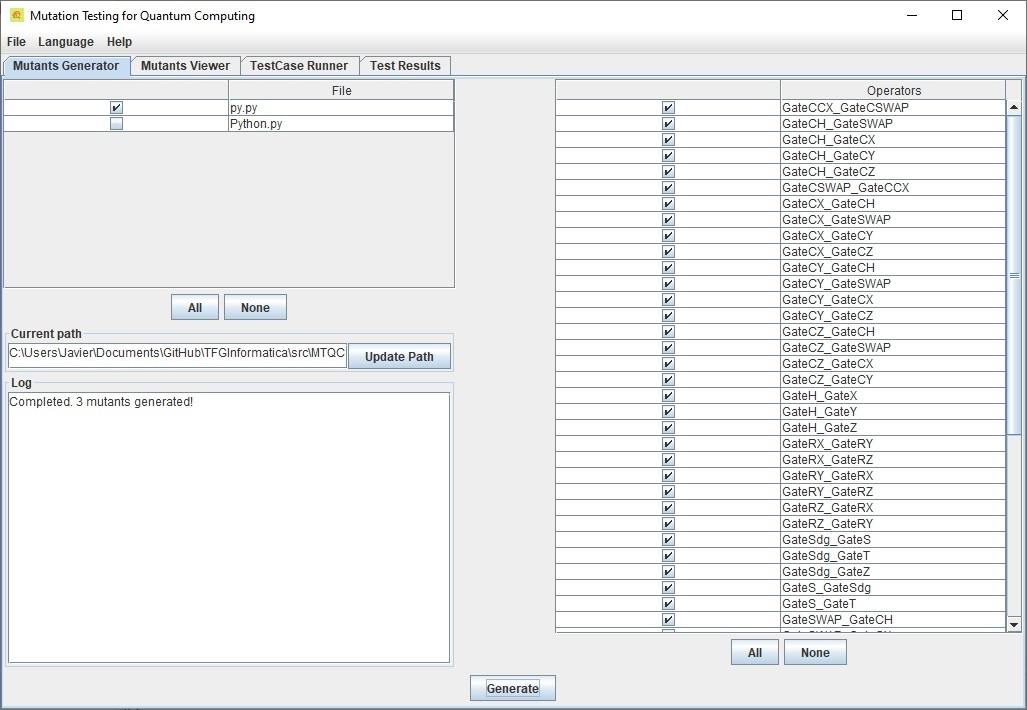
\includegraphics[scale=0.45]{images/vista1}
\end{center}
\caption{Vista del subsistema generador de mutantes.}
\label{fig:vista1}
\end{figure}

La generación de mutantes es el primer paso para realizar pruebas de mutación. En la figura \ref{fig:vista1} \ se contempla el aspecto de la vista asociada. La interfaz en su conjunto y cada una de las pestañas tiene un diseño simple, tratando de minimizar la cantidad de información para facilitar el uso y entendimiento del cliente.

Los componentes de esta vista se encuentran en el paquete view.mutantgeneratorview, aunque además hace uso de clases del paquete view.tools. En concreto, JTableCheck, que gestiona una tabla de  objectos de una determinada instancia junto a casillas verificadoras asociadas a booleanos y LogArea que imprime información para el usuario.

En cuanto a la lógica, los operadores se encuentran definidos todos ellos en el paquete model.mutantoperator, y los mutantes generados se gestionan para su uso en el resto del programa mediante la clase Mutant del paquete model.mutant.

La vista ofrece al usuario una lista de archivos en un determinado directorio que puede ser cambiado por el usuario. También aparece una lista de operadores de mutación acorde con en lenguaje cuántico seleccionado en ese momento. Tras la selección de los archivos y operadores se procede a llamar al controlador para que ordene a la lógica la creación de los mutantes.

Para la generación de mutantes se ha implementado la técnica del programador hábil, sólo se aplica una mutación a cada archivo generado. El proceso que sigue la lógica es sencillo, un operador contiene una secuencia de caracteres a ser buscada y otra con la que es reemplazada. Así, por cada archivo y operador, se generan tantos mutantes como veces se encontró dicha cadena. Todas estas acciones se realizan desde las clase Model.

De haber algún reto en esta fase del desarrollo, se trataría del hecho de establecer cuando hemos encontrado una cadena de caracteres coincidente con la mutación que queremos incurrir. En el caso de \textit{Qiskit} es sencillo, pues todas las instrucciones cuánticas son métodos que son llamados mediante un objeto perteneciente a la clase QuantumCircuit. Así, todas las instrucciones son del siguiente estilo

\begin{center}
objeto.instrucción(...)
\end{center}

y por tanto podemos buscar la cadena \textbf{.instrucción(} y sustituirla por \textbf{.mutación(} donde las palabras instrucción y mutación representan la conversión requerida. En el caso de \qsh\ no es tan sencillo, ya que las instrucciones tienen el aspecto de

\begin{center}
instrucción(...)
\end{center}

así que no basta con sustituir \textbf{instrucción(} por \textbf{mutación(}. Supongamos que queremos realizar mutantes cambiando el operador de la puerta de \textit{Hadamard}, representado por la instrucción H(...), por la puerta X, si en el proceso encontrásemos un método (por raro que fuera) acabado en H, por ejemplo applyH(...), estaríamos generando un mutante en el que esa instrucción sería cambiada por applyX(..) que no es el efecto que deseamos. La solución a esto es comprobar el carácter anterior y verificar que se trata de un salto de línea, un espacio o una tabulación.

Otro problema similar se aplica a los operadores de mutación aplicados a constantes en \qsh como \textbf{One} y \textbf{Zero}. La solución es, de nuevo, la comentada en el párrafo anterior pero aplicando dicha comprobación también al carácter posterior.

\subsubsection{Subsistemas: Visualizador de mutantes}

El segundo subsistema es el más simple de los cuatro. Se trata de una vista sencilla (figura \ref{fig:vista2}) que muestra la lista de mutantes generados y dos áreas de de texto, que actúan como \textit{display} de los ficheros original y mutante. Si no se han generado mutantes previamente, la lista aparecerá vacía.

\begin{figure}[htb]
\begin{center}
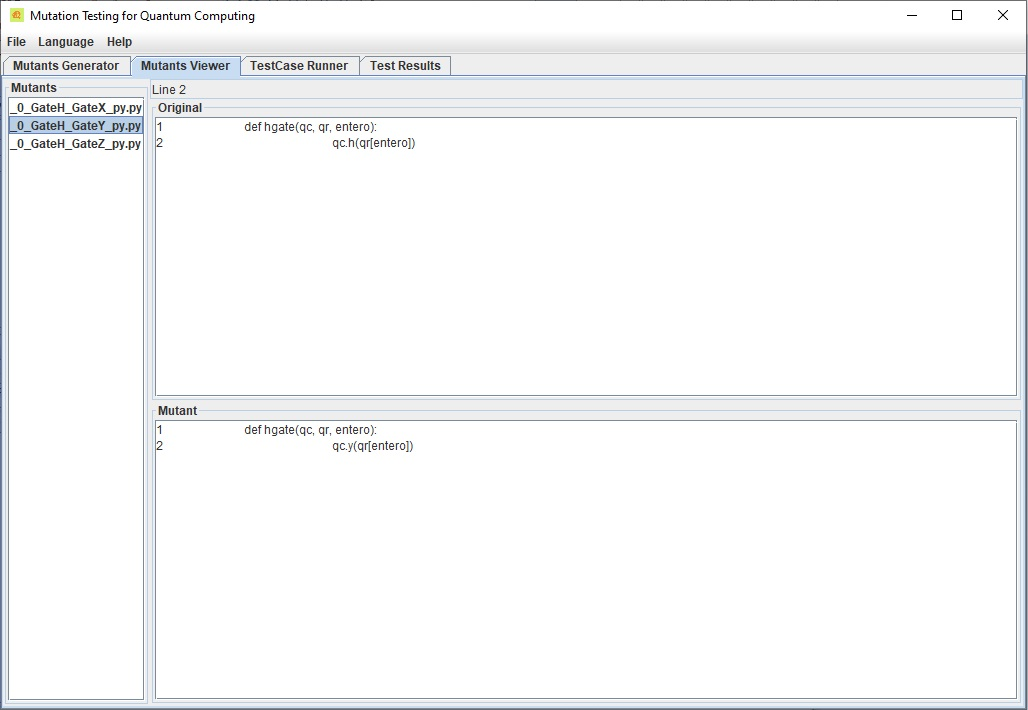
\includegraphics[scale=0.45]{images/vista2}
\end{center}
\caption{Vista del subsistema visualizador de mutantes.}
\label{fig:vista2}
\end{figure}

La lista de mutantes se gestiona mediante la clase JMutantList en el paquete view.tools. El resto de componentes se gestionan desde las clases FileArea y MutantsViewer del paquete view.mutantsviewer. Además, la lista antes mencionada contiene, no sólo el identificador del mutante, sino la instancia al completo.

El funcionamiento es sencillo, el usuario debe pinchar sobre el mutante que quiera ser observado y la vista puede obtener de dicho mutante las rutas a los archivos original y mutado sin necesidad de hacer llamada al controlador y, por tanto, tampoco al modelo. Tal vez en este caso no se esté siguiendo las directrices del patrón MVC como es debido, pero por su simplicidad optamos por este camino.

\subsubsection{Subsistemas: Pruebas de mutación y creación de test}

Es sin duda el componente más complejo del programa. En él intervienen gran parte de la lógica realizada para el proyecto. La funcionalidad se resume en ejecutar una elección de mutantes con unos casos de prueba determinados para decretar qué porcentaje de ellos ha sido matado y la eficacia de dichas pruebas.

\begin{figure}[htb]
\begin{center}
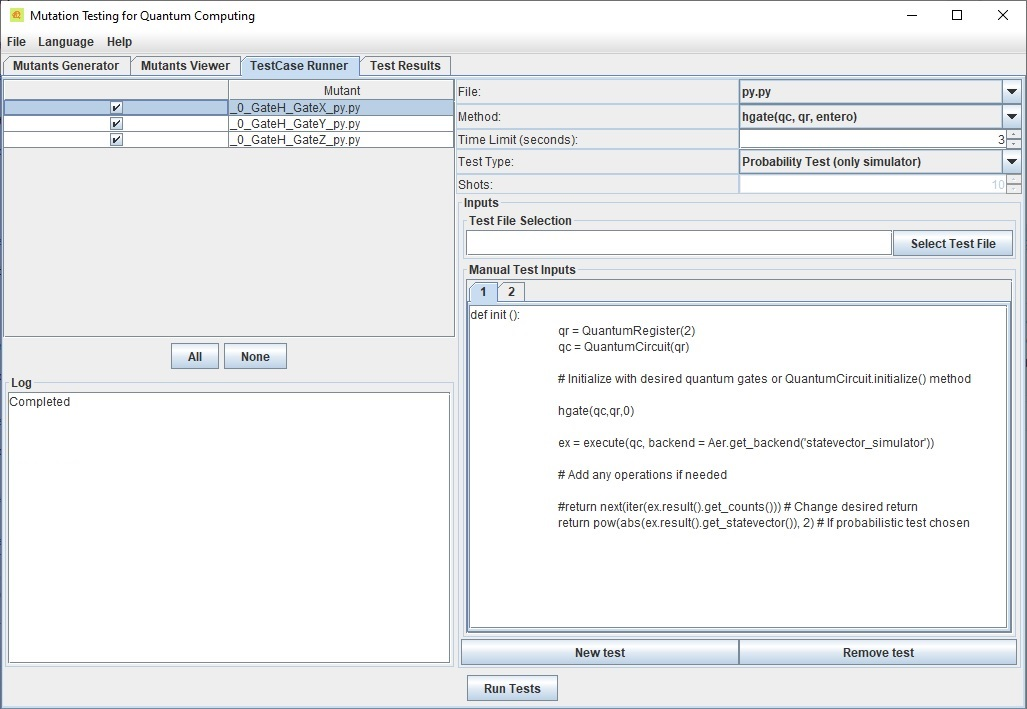
\includegraphics[scale=0.45]{images/vista3}
\end{center}
\caption{Vista del subsistema pruebas de mutación y creación de test.}
\label{fig:vista3}
\end{figure}

En la figura \ref{fig:vista3} tenemos la vista que constituye el subsistema cuyos componentes se engloban dentro del paquete view.testcaserunnerview y, además, hace uso de las clases del paquete view.tool TabbedTextArea, que gestiona las entradas para los casos de prueba que el usuario puede introducir mediante un sistema de pestañas; JTableCheck, tabla que gestiona la selección de mutantes; TextField, un simple campo de texto y LogArea, que imprime información de la ejecución del programa al usuario.

Aunque el usuario podía en el primer subsistema seleccionar más de un archivo para aplicar mutaciones sobre él, para realizar las pruebas de mutación debemos hacerlo, en este caso, de manera individual. Además, los archivos que MTQC genera para ejecutar todas las pruebas se almacenan en una carpeta auxiliar; Por tanto, el programa a probar no podrá usar archivos o librerías que no estén en el directorio por defecto del lenguaje correspondiente. Para solucionar esto, el usuario puede incluir la ruta a los archivos necesarios en el propio programa. Por ejemplo en \textit{Python} puede hacerse con

\begin{figure}[htb]
\begin{lstlisting}[language=Python]
import sys
sys.path.insert(0, "path_to_your_package")
\end{lstlisting}
\caption{Código para añadir una nueva ruta donde \textit{Python} buscará módulos.}
\label{fig:code1}
\end{figure}

aunque, en general, los programas cuánticos rara vez alcanzan una extensión suficiente para ser modulados en varios archivos y no debe ser un problema en la mayoría de casos.

Así, la primera decisión que ha de tomar el usuario es la de elegir el archivo deseado. En la vista se muestran los correspondientes a la ruta seleccionada en el primer subsistema. Tras la elección, se llama al controlador para que la lógica realice dos tareas. La primera es obtener todos los mutantes generados a partir del archivo seleccionado; la segunda es devolver todas las funciones encontradas en el archivo.

El usuario debe ahora realizar el resto de la configuración: Elegir los mutantes a ejecutar, la función de llamada, el tiempo límite para la ejecución de cada prueba (para evitar ejecuciones infinitas debido a que nos hayamos quedado en un bucle a causa de la mutación), el tipo de test, elegir el número de ejecuciones si este último es probabilista y , por último, las entradas o test.

En cuanto al tipo de test, está implementado uno determinista que hemos denominado \textbf{\textit{QStateTest}} y otro probabilista, \textbf{\textit{ProbabilisticTest}}. El primero compara las probabilidades arrojadas por los estados finales del sistema cuántico. Supongamos que una función sobre un sistema cuántico de un qubit devuelve $\frac{1}{\sqrt{2}}\ket{0}+\frac{1}{\sqrt{2}}\ket{1}$ mientras que el mutante devuelve $\frac{1}{\sqrt{2}}\ket{0}-\frac{1}{\sqrt{2}}\ket{1}$, este test evalúa las probabilidades de cada estado, que en ambos casos son de $\frac{1}{2}$ para $\ket0$ y un $\frac{1}{2}$ para $\ket1$. Por tanto no se mataría al mutante pese a que los estados cuánticos no son idénticos.

Sobra decir que este test solo es posible si se ejecuta sobre un simulador en un computador clásico. Para su implementación, en el caso de \qsh\ hemos hecho uso de la instrucción \textbf{DumpMachine()} que imprime en un fichero o pantalla el estado cuántico en ese momento, mientras que el simulador \textbf{StatevectorSimulator} de \textit{Qiskit} permite de igual modo acceder a dicha información.

El segundo tipo de test, \textit{ProbabilisticTest}, compara la salida final de la función que, generalmente, será la medición de uno o más qubits. Por tanto, esta salida puede ser probabilista y su ejecución puede ser realizada en repetidas ocasiones con el fin de conseguir una certeza estadística sobre la muerte o no del mutante. Dicho test puede ser aplicado en computadoras cuánticas usando \textit{Qiskit}, basta con seleccionar una máquina de \textit{IBM} disponible para la ejecución escribiendo el código correspondiente en la entrada. Sin embargo, hay que tener en cuenta que la disponibilidad de estas computadoras es muy limitada y las ejecuciones mensuales también lo son, así que podría demorar bastante tiempo.

Como vimos en el capítulo anterior, la inicialización del estado cuántico deseado supone un problema añadido respecto de la computación clásica. El usuario debe darnos una secuencia de puertas para conseguir el estado de entrada deseado. En el caso de \textit{Qiskit} existe una función del circuito cuántico (QuantumCircuit), \textbf{initialize()}, que permite inicializar el circuito en el estado deseado, siempre que el simulador utilizado sea StatevectorSimulator.

\begin{figure}[htb]
\begin{lstlisting}[language=Python]
from qiskit import *
import numpy as np

qr = QuantumRegister(3)
qc = QuantumCircuit(qr)
init = [complex(0, 1/np.sqrt(2)), 0, 0, complex(1/np.sqrt(2), 0), 0, 0, 0, 0]
qc.initialize(init, qr)
\end{lstlisting}
\caption{Inicialización de un circuito cuántico mediante un vector complejo en \textit{Qiskit}.}
\label{fig:code2}
\end{figure}

El código anterior inicializa el circuito cuántico de 3 qubits en el estado $\frac{i}{\sqrt{2}}\ket{000}+\frac{1}{\sqrt{2}}\ket{011}$. Nótese que el vector dado como ejemplo tiene norma uno; en otro caso la ejecución nos arrojaría un error.

En cualquier caso, la preparación de la entrada requiere un tratamiento previo. Para tratar esta entrada hemos facilitado dos métodos. El primero es mediante la carga de un archivo de texto en el que cada caso es separado por una línea con la secuencia de caracteres \textbf{***} y cada caso tiene que tener la estructura del segundo método que mencionamos a continuación. El segundo es un sistema de pestaña. Por defecto aparece una pestaña con un ejemplo estructural a seguir y en el caso de de añadir una nueva, aparece con una copia del contenido de la seleccionada previamente. El código dado por defecto para \textit{Qiskit} está reflejado en la figura \ref{fig:code3}.

\begin{figure}[htb]
\begin{lstlisting}[language=Python]
def init ():
	cr = ClassicalRegister(1)
	qr = QuantumRegister(1)
	qc = QuantumCircuit(qr, cr)

	# Initialize with desired quantum gates or QuantumCircuit.initialize() method

	# Call your method

	ex = execute(qc, backend = Aer.get_backend('statevector_simulator'))

	# Add any operations if needed
	
	return next(iter(ex.result().get_counts())) # Change desired return
	#return pow(abs(ex.result().get_statevector()), 2) # If probabilistic test chosen
\end{lstlisting}
\caption{Código dado por defecto en MTQC para inicializar un caso de prueba en \textit{Qiskit}.}
\label{fig:code3}
\end{figure}

Según lo deseado, podemos modificar el número de registro clásicos (\textbf{ClassicalRegister}) y cuánticos (\textbf{QuantumRegister}), añadir la inicialización deseada en cada caso y debemos llamar al método elegido. Por último, habrá que habrá que comentar uno de los dos \textit{return} en función al tipo de test elegido según se indica o incluso puede ser cambiado para devolver otro tipo de datos si se desea. Es importante recalcar que \textit{Qiskit} construye un circuito con el uso de métodos de aplicación de puertas, pero realmente ese circuito no se ejecuta hasta que no se llama a la instrución \textbf{execute(...)}. Si esta función es llamada durante el método que será probado, basta con comentar o borrar la línea de código correspondiente de la figura \ref{fig:code3}.

En cualquier caso, debemos mantener la tabulación establecida y no cambiar el nombre del método definido en la primera línea, pues es llamado para poder ser inicializada la entrada. Si es opta por la introducción vía archivo, este método tiene que estar definido para cada caso de igual modo.

\begin{figure}[htb]
\begin{lstlisting}[language=c++]
//Select desired Qubit number to be used
using (register = Qubit[2]) {

	//Inicialize variables and Qubits
	let count = 1;
	let initial = Zero;

	//Call method and save output
	let(output) =  method(...);

	//If probabilistic test chosen.
	//DumpMachine("temp.txt");

	//Reset all qubits to Zero state
	ResetAll(register);

	//Return output
	return output;
}
\end{lstlisting}
\caption{Código dado por defecto en MTQC para inicializar un caso de prueba en \qsh.}
\label{fig:code4}
\end{figure}

Las mismas indicaciones tenemos para \qsh\ (figura \ref{fig:code4}), debemos mantener la estructura general y modificar lo necesario siguiendo las indicaciones, ya haya sido elegido el método de entrada mediante el uso de la vista de pestañas o mediante la carga de archivo.

Tenemos así todo listo para proceder: archivo, método, mutantes, tipo de test y casos de prueba, entre otros. Todos estos datos se gestionan con las clases mencionadas anteriormente para cada uno de ellos. El usuario está listo para ejecutar los test, así, la vista llama al controlador que preprocesa los datos antes de mandárselos a la lógica. El primer objetivo es preparar nuevos archivos que añadan las entradas establecidas a los archivos a ejecutar: mutantes y original. Dichos archivos son creados por las clases del paquete model.language y gestionadas por la clase TestFile del paquete model.files.

El siguiente paso es generar un archivo principal en \textit{Python} que será ejecutado mediante una llamada al sistema (por tanto el usuario debe tener agregado \textit{Python} en su \textit{path}) y que llamará a todos los archivos generados en el paso anterior para obtener las salidas arrojadas por los test.

Tras ser ejecutados, MTQC recoge las salidas resultantes de la ejecución asignándolas al archivo original o mutante y a uno de los test según corresponda. Esta gestión de datos se realiza mediante una de las clases del paquete model.testresult según el tipo de test elegido.

Para acabar, todos los archivos generados durante esta fase son borrados y se manda una actualización de los resultados obtenidos al último subsistema que veremos a continuación.

\subsubsection{Subsistemas: Visualizador de resultados}

En último lugar tenemos el subsistema dedicado a visualizar los resultados. La vista (figura \ref{fig:vista4}) es un sencillo sistema de pestañas, una para cada test, que contiene una tabla donde se comparan los resultados y se indica qué mutantes han muerto y cuáles no.

Los componentes de la vista se encuentran íntegramente en el paquete view.testresultview a excepción de la clase ResultTable, que gestiona cada tabla, del paquete view.tools. Como hemos mencionado, los resultados que se muestran en esta vista se actualizan automáticamente al final de la ejecución del subsistema anterior.

\begin{figure}[htb]
\begin{center}
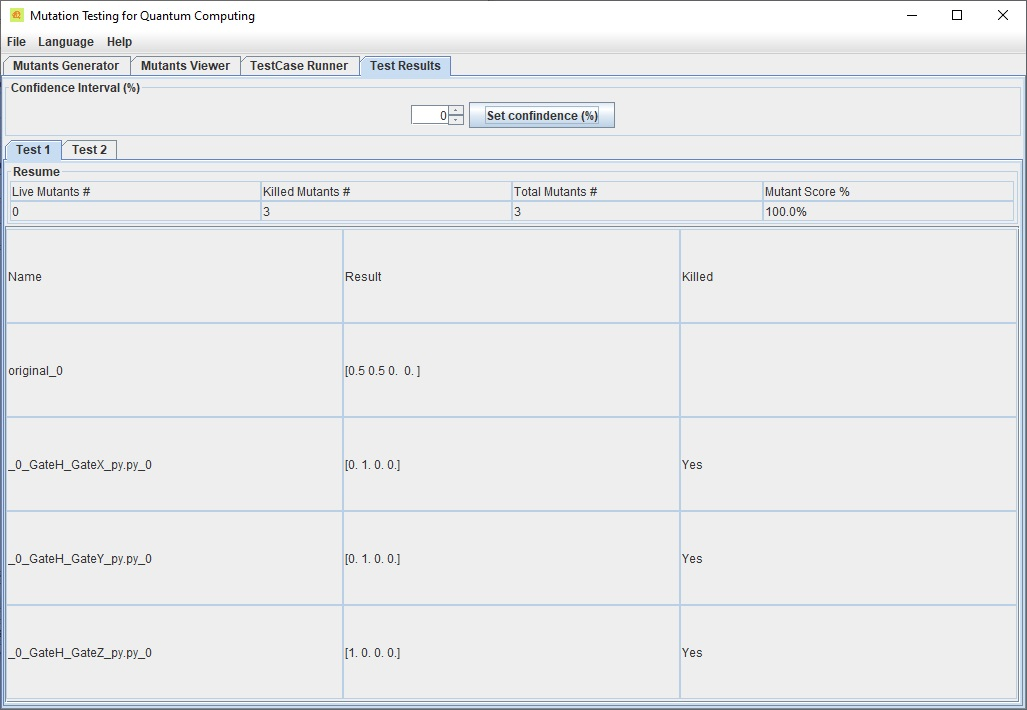
\includegraphics[scale=0.45]{images/vista4}
\end{center}
\caption{Vista del subsistema visualizador de resultados.}
\label{fig:vista4}
\end{figure}

Además, el usuario puede modificar la confianza utilizada para matar a un mutante en un test probabilístico, veamos como funciona. Supongamos que tenemos un total de $n$ estados posibles ($\ket0,...,\ket{n-1}$) en cierto sistema cuántico y hemos ejecutado $k$ veces tanto el archivo original como el mutante. Definimos las probabilidades de medición del estado cuántico $\ket i$ para el archivo original como

\begin{equation}
p_{\ket i,o}=\dfrac{f_{\ket i,o}}{k}
\end{equation}

donde $f_{\ket i,o}$ denota el número de veces que la salida del programa original fue el estado $\ket i$. Análogamente, para cierto archivo mutante $m$ definimos las probabilidades de medición del estado cuántico $\ket i$ como

\begin{equation}
p_{\ket i,m}=\dfrac{f_{\ket i,m}}{k}
\end{equation}

donde $f_{\ket i,m}$ denota el número de veces que la salida del mutante $m$ fue el estado $\ket i$. Así un mutante $m$ muere si se verifica

\begin{equation}
\max \{|p_{\ket i,o}-p_{\ket i,m}|:0\leq i\leq n - 1\}> c
\end{equation}

donde $c$ denota el parámetro de confianza que puede ser manipulado por el cliente. Obviamente el máximo del conjunto anterior está comprendido entre 0 y 1 por estarlo las probabilidades definidas anteriormente. El parámetro de confianza en MTQC por defecto es del 1\%, pero puede modificarse al porcentaje deseado. Tras esto, se contactará con la clase Model de la lógica que solicitará a cada instancia de la clase TestResult que recalcule la muerte o no del mutante en función del nuevo valor indicado y comunicará a la vista los resultados.
